\section{A Taxonomy of Replication Protocols}~\label{sec:tax}
% \todo{lin (spec) + diagrams, taxonomy based on writes, inline reads}

This section serves two purposes.
First, we present a taxonomy of strongly-consistent replication protocols.
The taxonomy will not only inform our choice of protocols to implement and evaluate, but will also enable us to generalize the results of each protocol to its respective class.
Second, we describe the operation of various protocols, providing the background material necessary for the rest of this paper.
Before diving into the taxonomy we first offer three remarks on the protocols and the corresponding jargon.

\beginbsec{Remarks}
Firstly, note that a lot of the protocols that we discuss can also execute transactions. However, this work will view them solely through the lens of the read/write API, explaining how each protocol performs a read and a write to keys stored in the replicated KVS.

Secondly, note that the problem of performing a conditional write in an environment where machines can fail and network/processing delays are unbounded is equivalent to asynchronous consensus~\cite{Herlihy:2008}. 
This is why some of the protocols we are studying are known under the umbrella of \qt{consensus protocols}. 
However, in this work we cast a wider net, investigating the sensitivity of performance to relaxing the fault model or to 
% In addition, we will also use ABD, to investigate the possibility of 
downgrading the API from conditional writes to plain writes.
For that reason we refer to the protocols discussed in this paper with the general term \qt{strongly-consistent replication protocols}.

Finally, note that throughout this paper, when we refer to a \qt{local read}, we refer to an operation that is performed by a machine that knows it is in the configuration and hence reads from its local KVS.  
% A machine can have that knowledge by maintaining a time lease that has not yet expired, by actively probing a configuration service~\cite{Dragojevic:2014}, or by maintaining per object leases~\cite{Chandra:2016}. In any of these cases the overhead (\eg of maintaining a lease) is amortized among millions of read operations and therefore we consider it to be zero.

\subsection{Taxonomy}

Our taxonomy is split into four quadrants as shown in \tabref{tab:tax} based on two operational patterns: 1) leader-based (L) vs. decentralized (D) and 2) total order (TO) vs. per-key order (PKO). Consequently, there are four resulting classes of protocols:
\squishenum
\item \emph{\LTO}: leader-based total order 
\item \emph{\LPKO}: leader-based per-key order
\item \emph{\DTO}: decentralized total order 
\item \emph{\DPKO}: decentralized per-key order
\squishenumend
% \antonis{Why not just use LT, LK, DT, DK instead? much easier for all these occurrences.}

\custvspace
Total order implies that protocols create a total order of all writes across all keys and apply them to the KVS in that order. In contrast, per-key order mandates that protocols only enforce a total order of writes at a per-key basis. 
Note that this does not affect the consistency guarantees;
in both cases, protocols can offer lin.
Leader-based protocols utilize a single node (\ie a leader) to enforce the ordering of the writes, while decentralized protocols achieve the same effect in a distributed manner.

\begin{table}[t]
\centering
\resizebox{0.48\textwidth}{!}{%
\begin{tabular}{c|c|c|}
\hhline{~--} %hline
& 
%%%%%%%%%%%%%%
\colorhl
\begin{tabular}[c]{@{}c@{}}

\textbf{Total order}

\end{tabular}      
& 
%%%%%%%%%%%%%%%%%%%%%
\colorhl
\begin{tabular}[c]{@{}c@{}}
\textbf{Per key order} \\ 

\end{tabular}
\\ \hline

\multicolumn{1}{|c|}{
\colorhl \textbf{
\begin{tabular}[c]{@{}c@{}}
Leader-\\ based 
\end{tabular} }}  & 
%%%%%%%%%%%
%% 
%%%%%%%%%%%
% \multicolumn{1}{c|}{
\begin{tabular}[c]{@{}c@{}}
    
    \textbf{Multi-Paxos}~\cite{Lamport:2001},
    \textbf{ZAB}~\cite{Hunt:2010, Reed:2008},\\
    VR~\cite{Oki:1988}, APUS~\cite{Wang:2017},
    DARE~\cite{Poke:2015},\\
    Raft~\cite{Ongaro:2014},
    Fast Paxos~\cite{Lamport:2006}
\end{tabular}
% }
& 
%%%%%%%%%%%

%%%%%%%%%%%
\begin{tabular}[c]{@{}c@{}}  
    \textbf{CHT}~\cite{Chandra:2016},
    FGSMR~\cite{Liu:2020}, \\
    WPaxos~\cite{Ailijiang:2020}, 
    Primary-backup~\cite{Alsberg:1976},\\
    CR~\cite{VanRenesse:2004},
    \textbf{CRAQ}~\cite{Terrace:2009},
\end{tabular}                                                                                                                                                                                                \\ \hline
\multicolumn{1}{|c|}{
\colorhl \textbf{\begin{tabular}[c]{@{}c@{}}
Decentralized \\ (Leaderless)
\end{tabular}}}
& 

\begin{tabular}[c]{@{}c@{}}
Mencius~\cite{Mao:2008},
    \textbf{Derecho}~\cite{Jha:2019},\\
    AllConcur~\cite{Poke:2017}
\end{tabular}
%%%%%
& 
\begin{tabular}[c]{@{}c@{}}
\textbf{CP}~\cite{Lamport:1998},
RMW-Paxos\cite{Skrzypczak:2020},\\
CASPaxos\cite{Rystsov:2018}
 Gryff~\cite{Burke:2020},\\
 Generalized Paxos~\cite{Lamport:2005}, 
 EPaxos~\cite{Moraru:2013},\\
 
 Atlas~\cite{Enes:2020},
 \textbf{All-aboard Paxos}~\cite{Howard:2019} \\
 \textbf{ABD~\cite{Lynch:1997}}, 
 \textbf{Hermes}~\cite{A:2020} \\
\end{tabular} 

\\ \hline
\end{tabular}%




}
\caption{Taxonomy (implemented protocols are in bold)}
\label{tab:tax}
\end{table}



% \begin{table}[t]
% % \small
% \footnotesize
% % \scriptsize
% %  \tiny
% \centering
% \resizebox{0.48\textwidth}{!}{%
% \begin{tabular}{|c|l|l|}
% \hline
% \multicolumn{2}{|c|}{\colorhl\textbf{Class}} &
% \multicolumn{1}{c|}{\colorhl\textbf{Protocols}}   
% \\ \hline
% %Dare, Sift, Apus, NoPaxos, Netchain

% \multirow{4.1}{*}{
% \begin{tabular}[c]{@{}c@{}}   Total-\\order\end{tabular}
% } & 
% \multicolumn{1}{c|}
% {\scriptsize \begin{tabular}[c]{@{}c@{}}   Leader-\\based\end{tabular} }  
% & 
% \multicolumn{1}{c|}{
% \begin{tabular}[c]{@{}c@{}}
%     \textbf{ZAB}~\cite{Hunt:2010, Reed:2008},
%     \textbf{Multi-Paxos}~\cite{Lamport:2001},\\
%     VR~\cite{Oki:1988},
%     Raft~\cite{Ongaro:2014},
%     Fast Paxos~\cite{Lamport:2006}\\
% \end{tabular}
% }
% \\ \cline{2-3}
% & 
% \multicolumn{1}{c|}{
% \scriptsize \begin{tabular}[c]{@{}c@{}}   
% per-key\\order
% \end{tabular} 
% } &
% \multicolumn{1}{c|}{
% \begin{tabular}[c]{@{}c@{}}  
%     \textbf{CHT}~\cite{Chandra:2016},
%     FGSMR~\cite{Liu:2020}, \\
%     Primary-backup~\cite{Alsberg:1976},
%     CR~\cite{VanRenesse:2004},\\
%     CRAQ~\cite{Terrace:2009},
% \end{tabular} 
% }

% \\ \hline
% %%%%%%%%%%%%%%%%%%%%%%%%%%%%%%%
% %  

% % \begin{tabular}[c]{@{}c@{}}Rotating \\ Leaders   \end{tabular}   & 
% % \begin{tabular}[c]{@{}c@{}}
% % Mencius~\cite{Mao:2008},\\
% %     Derecho~\cite{Jha:2019},
% %     AllConcur~\cite{Poke:2017},
 

% % \end{tabular}

% % \\ \hline
% \multirow{4.1}{*}{Leaderless} & 
% \multicolumn{1}{c|}{
% \scriptsize 
% \begin{tabular}[c]{@{}c@{}}   
% static\\order
% \end{tabular} 
% }
% & 
% \multicolumn{1}{c|}{
% \begin{tabular}[c]{@{}c@{}}
% Mencius~\cite{Mao:2008},\\
%     \textbf{Derecho}~\cite{Jha:2019},
%     AllConcur~\cite{Poke:2017},
% \end{tabular}
% }
% % \\ \hline

% \\ \cline{2-3}
% & \multicolumn{1}{c|}{
% \scriptsize 
% \begin{tabular}[c]{@{}c@{}}   
% dynamic-\\order
% \end{tabular} 
% } &
% \multicolumn{1}{c|}{
% \begin{tabular}[c]{@{}c@{}}
% \textbf{Classic Paxos}~\cite{Lamport:1998},
%  Gryff~\cite{Burke:2020},
%  EPaxos~\cite{Moraru:2013},\\
%  Generalized Paxos~\cite{Lamport:2005}, 
%  Atlas~\cite{Enes:2020},\\
%  \textbf{All-aboard Paxos}~\cite{Howard:2019} 
%  \textbf{Hermes}~\cite{A:2020} \\
% \end{tabular} 
% }
% \\ \hline
% \end{tabular}
% }
% \caption{Classification of  protocols.}
% \label{tab:tax}
% \end{table}

Why choose these two axes to categorize protocols?
We hypothesize that from a performance perspective, protocols must optimize for three metrics: 
1) thread-scalability: the protocol's ability to scale with more threads, 
2) load-balance: whether the work required to complete a request is evenly distributed among all nodes and 
3) the work-per-request ratio: the total cpu, network and memory resources required to complete a single request.

The classification is derived from the above three metrics.
Specifically, total order protocols---with or without a leader---struggle to achieve thread-scalability because applying writes in order requires coordination between the threads. 
Leader-based protocols struggle to achieve load balance as the leader tends to carry out most of the work required to execute a write. 
Both techniques (leader and total order)
help reduce the work-per-request ratio as they provide an easy way to serialize writes.
Conversely, protocols that are both per-key and leaderless tend to require a higher work-per-request ratio because the protocols must do additional work to serialize writes in a distributed manner.
% Finally, protocols that are both per-key and leaderless tend to require a higher work-per-request ratio
% simply because they can use neither a total order of writes nor a leader to serialize writes. 
We will substantiate these claims in our evaluation section (\S\ref{sec:ev}).
% \todo{Should the metrics be revisited, as classes are explained??}

% Below, we will first briefly summarize how protocols from each class can perform writes and reads and then in the next section we will address their availability guarantees and how they factor in the performance discussion.

% \begin{figure}[t]
  \centering
  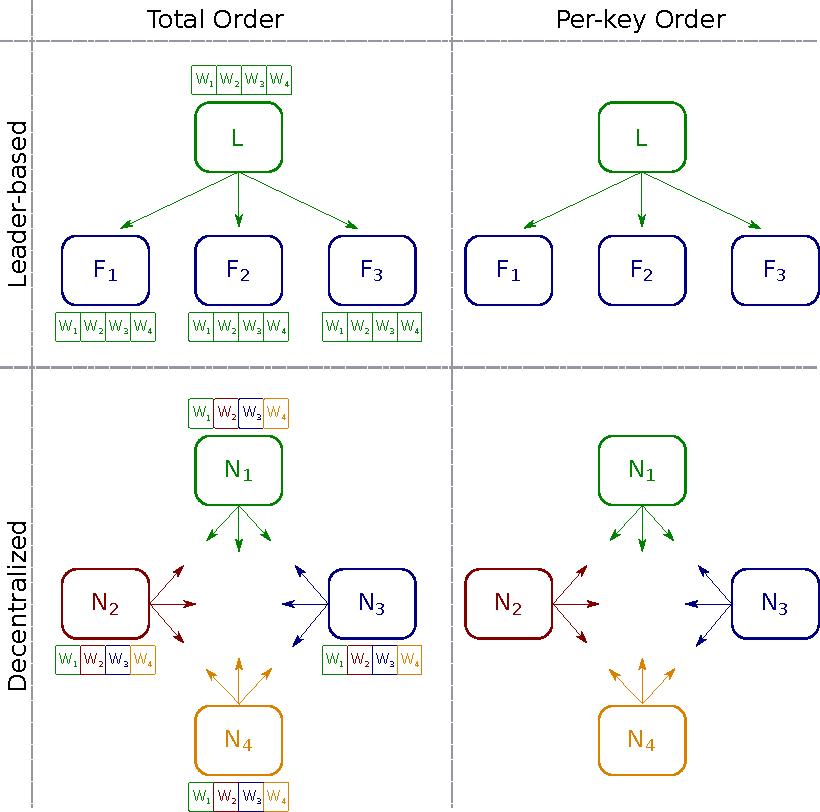
\includegraphics[width=0.45\textwidth]{1_figures/tax-fig.pdf}
%   \vspace{-0.5em}
  \caption{The operational pattern of the four classes. In leader-based protocols a leader (L) propagates writes to the followers (F1-F3). 
  In decentralized protocols, all nodes (N1-N4) propose writes.
  In total order protocols, a total order of writes is maintained in each node.}
%   \vspace{-1.5em}
  \label{fig:tax}
\end{figure}

% \subsection{Leader-based protocols}
% We start the discussion with the two leader-based classes, \LTO~and \LPKO. We first see how each class can perform writes, then discuss reads for both classes and finally will reason about the protocols we chose to implement and evaluate.


% \beginbsec{\LTO}
\subsection{Leader-based \& Total Order (\LTO)}\label{sec:tax:lto}
% \beginbsec{Writes}
Protocols such as ZAB~\cite{Hunt:2010}, Multi-Paxos~\cite{Lamport:2001} and Raft~\cite{Ongaro:2014} serialize \emph{all} writes at the leader node, creating the total order. The leader executes the writes by proposing them to the rest of the nodes (dubbed \emph{followers}), typically in two broadcast rounds: a \emph{propose} round to which followers respond with an acknowledgement (ack), and a \emph{commit} round. All nodes must apply committed writes in their total order.  

\beginbsec{Reads}
A write is guaranteed to propagate to only a majority of nodes. The leader is the
only node that is guaranteed to be in that majority, and thus the only node guaranteed to know of the latest committed write for any key.
%is the leader, and the leader is guaranteed to be in that majority.  
%but  which includes the leader. 
% Thus, the leader is the only node that is guaranteed to know of the latest committed write for any key. 
As such, the leader can always read locally.
Followers must send their reads to the leader, querying it for the latest value.

There are two possible relaxations that allow local reads in follower nodes, too. 
The first relaxation is to simply forego linearizability, conceding that reads may not return the latest write. This is tolerable 
% \antonis{tolerable doesn't seem a great word here. Maybe feasible/achievable.}
for \LTO~protocols, because if writes are totally ordered, this relaxation downgrades consistency guarantees only mildly to Sequential Consistency~\cite{LevAri:2017}. ZAB subscribes to this practice.

The second relaxation that allows followers to read locally is to 
ensure that every write reaches all followers. 
% CHT and CRAQ~\cite{Terrace:2009}, an optimized variant of CR, exemplify this relaxation. 
Note that there is a downside in requiring that all writes propagate to \emph{all} nodes: even if one node fails, all writes block. We elaborate in \secref{sec:fail}.

\beginbsec{Choices}
To represent \LTO, we implement ZAB and Multi-Paxos (MP), capturing the difference between local reads (with relaxed consistency) and linearizable reads that must be sent to the leader node.
% The performance of protocols such as Raft will be captured by MP~\cite{Howard:2020}.

% The same relaxation in an \LPKO~protocol would result in very weak guarantees (\ie Eventual Consistency~\cite{Vogels:2009}) that are beyond the scope of this work.
% Therefore this relaxation is only applicable for \LTO~protocols; in \LPKO~protocols reading locally 

\subsection{Leader-based \& Per-key Order (\LPKO)}\label{sec:tax:lpko}
% \beginbsec{\LPKO}

% \beginbsec{Writes}
Protocols in this class use the leader node to only serialize writes \emph{to the same key}. Specifically, all writes are steered to the leader node, which simply ensures that writes to the same key are applied in the same order by all replicas. A typical example of this class is the CHT~\cite{Chandra:2016} protocol, where the leader executes writes in two rounds as described in the total order class. 
There are two possible optimizations protocols can employ.

The first is exemplified by Chain Replication (CR)~\cite{VanRenesse:2004}. In CR, the leader does not broadcast the writes to the followers; rather the nodes are organized in a chain, through which writes propagate from the head of the chain to its tail. The head node acts as the leader in that all writes have to be steered to it so that it serializes them. In our evaluation, we will see how this approach significantly---but not entirely---alleviates the load balance problem.

The second optimization also tackles load balance, by denoting that all nodes are leaders for a subset of the keys. For example, for a 5-node deployment the key space is partitioned five ways, where each node is denoted leader for only one of the partitions.
Notably, this is possible in \LPKO---but not \LTO---because the leader need not enforce an order across all writes. %The optimization was recently proposed in the FGSMR paper~\cite{Liu:2020}.

\beginbsec{Reads}
\LPKO~protocols can execute lin reads in the same manner as \LTO~protocols. %which depends on write propagation. 
When writes propagate to a majority of nodes, reads have to be propagated to the leader. When writes are guaranteed to propagate to all followers, reads can execute locally in all nodes. CHT and CRAQ~\cite{Terrace:2009}, an optimized variant of CR, both subscribe to this approach.

Finally, note that the option to propagate writes to a majority of nodes but execute reads locally by  downgrading consistency to SC (discussed for \LTO) is not available for per-key order protocols. Reading locally in this case would result in very weak guarantees (\ie Eventual Consistency~\cite{Vogels:2009}).

\beginbsec{Choices}
To represent \LPKO, we implement three protocols: CHT, CRAQ and a variant of CHT with multiple leaders, dubbed \emph{CHT-multi-ldr}. 
CHT represents the typical \LPKO~protocol, 
%but also allows for local reads.
CRAQ captures the CR optimization for load balancing writes and %, plus it also allows for local reads in all nodes. 
finally, CHT-multi-ldr captures the optimization of denoting all nodes as leaders of a partition of the key space.
All three protocols read locally.
%but unlike FGSMR, it can also perform local reads.



\begin{comment}


\beginbsec{Reads in \LTO~and \LPKO}
A write is only guaranteed to propagate to a majority of nodes, which includes the leader. Therefore, the leader is the only node that is guaranteed to know of the latest committed write for any key. 
As such, the leader can always read locally. 
Followers must send their reads to the leader, querying it for the latest value.

There are two possible relaxations that allow local reads in follower nodes, too. 
The first relaxation is to simply forego linearizability, conceding that reads may not return the latest write. This is tolerable for \LTO~protocols, because if writes are totally ordered, this relaxation downgrades consistency guarantees only mildly to Sequential Consistency~\cite{LevAri:2017}. The same relaxation in an \LPKO~protocol would result in very weak guarantees (\ie Eventual Consistency~\cite{Vogels:2009}) that are beyond the scope of this work.
% Therefore this relaxation is only applicable for \LTO~protocols; in \LPKO~protocols reading locally 
ZAB subscribes to this practice.

The second relaxation, that allows followers to read locally, is to 
ensure that every write reaches all followers. 
CHT and CRAQ~\cite{Terrace:2009}, an optimized variant of CR, exemplify this relaxation. Note that there is a downside in requiring that all writes propagate to \emph{all} nodes: if one node fails, then all writes must to block. We elaborate in \secref{sec:fail}.


\beginbsec{Choices}
To represent \LTO, we implement ZAB and Multi-Paxos (MP), capturing the difference between local reads (with relaxed consistency) and linearizable reads that are sent to the leader node.
The performance of protocols such as Raft will be captured by MP~\cite{Howard:2020}.

\custvspace
To represent \LPKO, we implement three protocols: CHT, CRAQ and a variant of CHT with multiple leaders, dubbed \emph{CHT-multi-ldr}. 
CHT captures the generic case, plus it enables local reads.
CRAQ captures the CR optimization for load balancing writes, plus it also allows for local reads in all nodes. 
%whereas in vanilla CR, only one node -- the chain of the tail -- can read locally.
Finally, CHT-multi-ldr captures the optimization of denoting all nodes as leaders of a partition of the key space, but unlike FGSMR, it can also perform local reads.
\end{comment}
% \subsection{Decentralized protocols}
% We now dive into the operation of decentralized (\ie leaderless) protocols.

\subsection{Decentralized Total Order (\DTO)}\label{sec:tax:dto}
In \DTO\ protocols, the total order of writes is not created in a central location. Rather, 
there is typically a predetermined static allocation of write-ids to nodes. For example, 
all nodes know that the writes $0$ to $N - 1$ will be proposed and coordinated by node-0, the next $N$ writes (\ie $N$ to $2N - 1$) will be proposed by node-1 and so on.
Therefore, each node can calculate the place of each write in the total order based on its own node-id, without synchronizing with any other node. Then, the node broadcasts its writes along with their place in the total order. Typically a commit message is broadcast after gathering acks from a majority of the nodes.
Crucially, all nodes must apply the writes in the prescribed total order.
% An intuitive way to think of this operational pattern is imagine that nodes alternate as leaders in a round-robin fashion. This is why
% these protocols are also known as \qt{rotating coordinator protocols}.
% However, nodes need not actually rotate; they can execute their writes in parallel, as long as each nodes commits them in order.
Derecho~\cite{Jha:2019}, AllConcur~\cite{Poke:2017} and Mencius~\cite{Mao:2008}, all belong to the \DTO~class.

\beginbsec{Reads}
Reads can be executed 
% \antonis{via coordination (?)} 
by allocating slots in the total order, similarly to writes.
Local reads are also possible, either by downgrading consistency guarantees to SC (similarly to \LTO), or by enforcing that all writes will propagate to all nodes.
% Similarly to \LTO, there are two options for the reads.
% The first option is to Local reads by downgrading consistency guarantees to SC or enforcing that all writes propagate to all nodes. 
% Local reads will downgrade the If downgrading the consistency guarantees to SC is acceptable, reads can be executed locally in all nodes. Otherwise, lin can be enforced %by simply treating reads similarly to writes, i.e., 
% by allocating a slot for reads in the total order.

\beginbsec{Choices}
To represent \DTO, we implement and evaluate Derecho. In order to get the upper bound of the \DTO~class, we implement the Derecho variant that executes reads locally, downgrading consistency guarantees to SC.
%  To evaluate these protocols, we have built a prototype that models Derecho over \odlib.

\subsection{Decentralized Per-key Order (\DPKO)}\label{sec:tax:dpko}
In the fourth and final quadrant, \DPKO~protocols %dynamically \antonis{It seems a bit odd that DTO is presented as "static" (\S~3.4) and DPKO as "dynamic"} 
agree on a per-key order of writes in a distributed manner. There is no central leader---rather any node can propose and coordinate a write. 
The most prominent example is Classic Paxos (CP)~\cite{Lamport:1998}.
Traditionally, CP has been regarded simply as a way to perform leader election so that Multi-Paxos can start executing.
However, recent proposals~\cite{Skrzypczak:2020, Rystsov:2018, V:2020}
have used CP to reach consensus on which node should be the next to perform a write at a per key basis.

% perform writes (explicitly targeting conditional writes). 
% where nodes reach consensus on which node should be the next to perform a write at a per key basis. 

% has not been widely used to perform writes. This is because in Lamport's original paper it was not described how to run CP repeatedly. %, but we must be able to modify the same object multiple times.
% Rather, it was suggested that CP can be executed once to establish a leader which can then make all decisions (\ie Multi-Paxos).
% However, %the paper did note that it is possible to run CP without a log over a KVS. R
% recent proposals~\cite{Skrzypczak:2020, Rystsov:2018, V:2020} have presented enhancements to CP enabling it to run repeatedly in order to support writes. 

Notably, CP extracts a steep price: it requires three broadcast rounds to complete (propose, accept and commit~\cite{Howard:2019}), each of which contains considerably more metadata than any other protocol we have discussed, while responding to a propose or accept is also very complicated, as there are various possible responses, depending on the state of other conflicting ongoing writes. Finally, depending on conflicts, CP may have to retry an unbounded number of times~\cite{Fischer:1985}. 
%we would require three broadcast rounds~\cite{V:2020}.

The source of CP's overhead stems from the combination of three constrains:
1) conflicting writes may be concurrently executing at all times \emph{and}
2) it is impossible to guarantee that a message will always be delivered to all nodes \emph{and}
3) writes are conditional (\ie RMWs).
Relaxing any of the constraints will significantly simplify the problem.
Consequently, there are three approaches to optimize CP, one for each constraint.
The first approach is exemplified by protocols such as EPaxos~\cite{Moraru:2013}, Atlas~\cite{Enes:2020} and All-aboard Paxos~\cite{Howard:2019}, which provide a fast path, where consensus can be achieved after two broadcast rounds (accept and commit), 
in the absence of conflicts, 
using CP as the fallback option when conflicts do occur.
% All-aboard achieves
% All-aboard differs from EPaxos and Atlas, in that it does not require active

The second approach is presented by Hermes~\cite{A:2020}, which, similarly to CR and CHT, 
% \antonis{-- but in decentralized manner (?)}
enforces that a message will always be delivered to all nodes. With this guarantee, performing a write can be done in two lightweight broadcast rounds which are roughly equivalent to accept and commit. %Similarly to CR and CHT, Hermes must concede that if one node fails all writes must block, threatening the system's availability. We elaborate more in \secref{sec:fail}.


Finally, the third approach downgrades the API, offering plain writes instead of conditional writes.
%which is to maintain both constraints, but not perform consensus. In that case, it is the API that is getting sacrificed, as conditional writes cannot be supported, only regular writes.
Multi-writer ABD~\cite{Lynch:1997} is a variant of the ABD protocol~\cite{Attiya:1994} that exemplifies this approach. From now on, we refer to multi-writer ABD simply as ABD. 
A write in ABD requires two broadcast rounds that must reach a majority of nodes.

\beginbsec{Reads}
In \DPKO~protocols that do not guarantee that a write reaches all nodes, 
%as a majority suffices. Therefore 
there is no master copy to read from. 
Therefore, to get the most recently committed write, a read must consult a majority of nodes~\cite{Charapko:2019}. The reads should then perform a second round to ensure that the write is committed to a majority of nodes, so that subsequent reads can also observe it. 
We refer to this as the \emph{ABD-read} as it was first proposed in the original ABD protocol~\cite{Attiya:1994}. Notably, if writes are guaranteed to reach all nodes, reads can be performed locally.

\beginbsec{Choices}
To represent \DPKO~we implement and evaluate four protocols: CP, All-aboard, Hermes and ABD. CP will provide a baseline. 
All-aboard shows the limit of CP while maintaining its availability guarantees.
Hermes will show us the performance gains possible when writes reach all nodes. ABD will showcase the performance difference between conditional and regular writes. 

Notably, instead of All-aboard, we could have selected EPaxos~\cite{Moraru:2013} (or its most recent variant, Atlas~\cite{Enes:2020}). EPaxos requires that nodes respond to accept messages with recent conflicting commands. This requires memory, compute and network resources to store, retrieve, reply and transmit an unbounded number of conflicting writes.
In contrast, All-aboard is a zero-cost optimization. 
Specifically, All-aboard leverages the Flexible Paxos~\cite{Howard:2018} theorem to shave off the first round (propose) and significantly reduce the size of the commit round, without incurring a counterweight cost.
The complete specification of our All-aboard implementation over CP can be found in~\cite{Paxos-spec}.
% We intend to open-source the complete specification of our All-aboard implementation over CP.
% \antonis{I think this sentence is to be replaced with a link(?).}




% Finally, the recently proposed Hermes~\cite{A:2020} protocol represents the final design point in the space. Hermes assumes a stable configuration, and therefore assumes that any broadcast message will be delivered to all machines in said stable configuration. This allows Hermes to both perform RMWs in two broadcast rounds and perform reads locally. However, in the event of a failure Hermes must halt until the failed machine is safely removed from the configuration.

\subsection{The Impact on Availability}\label{sec:fail}
In this section, we discuss the implications of protocol design choices on the availability guarantees.








\begin{table}[t]
\centering
\resizebox{0.48\textwidth}{!}{%
\begin{tabular}{c|c|}
\hhline{~-} %

& \multicolumn{1}{|c|}{\colorhl Availability guarantees}
\\ \hline

 
\multicolumn{1}{|c|}{ \colorhl
\begin{tabular}[c]{@{}c@{}}
CP, ABD, All-aboard
\end{tabular}} & 

\multicolumn{1}{|c|}{ Always available}
\\ \hline


\multicolumn{1}{|c|}{ \colorhl ZAB, MP} &

\multicolumn{1}{|c|}{
\begin{tabular}[c]{@{}c@{}}
Unavailable for the duration of a \\ predefined time-out after the leader node fails 
\end{tabular}} 
\\ \hline


\multicolumn{1}{|c|}{ \colorhl
\begin{tabular}[c]{@{}c@{}}
Hermes, CRAQ, CHT, \\ CHT-multi-ldr, Derecho
\end{tabular}} &
\multicolumn{1}{|c|}{ 
\begin{tabular}[c]{@{}c@{}}
Unavailable for the duration of a \\ predefined time-out after any node fails
\end{tabular}} 

\\ \hline
\end{tabular}
}
\caption{\y{A summary of the availability guarantees of the \pnum\ protocols, with up to $f$ failures (with $2f + 1$ nodes). }}
\label{tab:avail}

\end{table}
% Our analysis has not considered the impact on availability of the various optimizations.
% There is an elephant in the room in our analysis: availability.

CP, All-aboard and ABD offer the highest level of availability guarantees.
Specifically, they assume the possibility of: 
1) non-Byzantine machine and network failures; and 
2) unbounded delays in both processing and networking. 
Under these assumptions, as long as $N/2 + 1$ nodes remain alive, responsive and connected, these three protocols will operate without interruption, \ie they will remain available.
% All-aboard and ABD provide the same guarantees, but the rest of the protocols do not.
The rest of the protocols that we have selected 
make design choices that downgrade these availability guarantees.


Specifically, leader-based protocols (ZAB, MP, CRAQ, CHT and CHT-multi-ldr)  will block if the leader becomes unresponsive.
Similarly, assuming that writes always reach all nodes (as in Hermes, CRAQ, CHT, and CHT-multi-ldr) results in blocking if any node becomes unresponsive.
Note that assuming that writes reach all nodes is a prerequisite for  linearizable local reads. Therefore, lin local reads can only be implemented at the expense of availability.
% Hermes and CRAQ assume that a write must be propagated to all nodes, and thus will block if any node becomes unresponsive.
% \todo{perhaps a footnote about CHT to preempt}
% In CHT, followers will block if the leader becomes unresponsive and the leader will block if any of the followers becomes unresponsive (alas in a slightly different manner than Hermes and CRAQ, as in CHT followers maintain read-leases at a key granularity).
Finally, Derecho assumes that every node makes use of their pre-allocated slots in the total order in a timely manner. If any node is slow to broadcast new writes, then all nodes will block.
\y{\tabref{tab:avail} provides a brief summary of the availability guarantees of the \pnum\ protocols.}


In all the above cases, a failure causes blocking for the duration of a predefined time-out. Expending this time-out will trigger a recovery action (\eg leader election, reconfiguration etc.). Once recovery is complete, operation can resume. 
The unavailability period is the sum of the length of the time-out plus the latency of the recovery action. 
% \antonis{Optionally you may say that the former tends to be the dominant latency.}\vasilis{I want to avoid this because for some it will  be controversial, and there is no need to go there}

This work provides a detailed performance analysis of replication protocols without delving into the nuances of availability. However, having pointed to the choices that come at the expense of availability, we enable the operator to select (or design) the protocol that best fits their needs.

% \antonis{On the other hand, regarding availability all-acks protocol have the benefit of N+1 (vs. 2N+1) replicas for to tolerate N faults if they use an external membership service. I think that's a key reason that in industry they use primary-backup/chain replication.} \vasilis{this opens up the CAP can of worms, we dont need this kind of level of detail}

\begin{comment}


% We form four groups to capture the behaviour of the remaining protocols.
% The first group contains ZAB and MP, which will block if the leader becomes unresponsive. The first follower that times-out on the unresponsive leader will trigger a new leader election.

% The second group consists of  CRAQ and Hermes, which assume that a write must be propagated to all nodes, and thus they will block if any node becomes unresponsive. In that case, nodes must first time-out and then remove the unresponsive node from the configuration, before they can resume operation. 

% The third group contains CHT and CHT-multi-ldr. 
% If the leader becomes unresponsive, then leader election must be triggered similarly to ZAB, MP. If 
% In CHT, the leader shares a lease with every other 
% %In addition, they require loosely synchronized clocks, so that different nodes can  to be able to agree on 
% Finally, Derecho assumes that every node will timely make use of their pre-allocated slots in the total write order. If any node is too slow to broadcast new writes, then all nodes will have to block.



% Not all cases are the same, CHT, CHT-multi-ldr, CRAQ and Hermes require loosely synchronzied clocksIn all cases, protocols will use a time-out
\vasilis{Up to here}

This work attempts to zero in on the performance of protocols.% abstracting away their failure guarantees.
However, it is not possible to completely isolate the performance of a fault-tolerant protocol from its availability guarantees.
% However, several operational aspects of a protocol are intertwined  with the availability it provides. To address that, 
Below, we provide a detailed record of how failure guarantees affect the operation of protocols.

When a machine crashes it typically creates a small period of unavailability. The live machines time-out on the failed machine and then perform the necessary actions to continue operation without the failed node. The length of the time-out is what determines the period of unavailability. The time-out's length must be chosen as a function of three things 1) the protocol-specific cost of a false positive  2) the availability guarantees the system must provide and 3) system specific timing restrictions that may cause false positives.
Of the three, only the first factor is protocol specific, the other two rest on the datacenter operator. 
Let us discuss the protocol-specific cost of a false positive by grouping protocols with similar behaviour.


In protocols such as Hermes, CR and CRAQ, a write must be seen by \emph{all} machines. When a machine fails, the rest of the machine must detect the failure and remove the machine from the configuration. Here the cost of a false positive is big because 1) the machine that was removed must be added again and go through a recovery phase and 2) consecutive false positives may lead to removing more than half the nodes from the configuration. Therefore, the time-out must be large enough to avoid false positives. However, in the event of a failure, that large time-out will create an equally large period of unavailability.

In leader-based protocols that only gather a majority of responses in order to complete a request (\eg ZAB, multi-Paxos, Raft), the failure of a follower machine does not need to be detected on the critical path of the request. It can be detected in the background, without causing any unavailability penalty. However, when it is the leader that becomes unresponsive, the rest of the followers must time-out on it and elect a new leader. The availability penalty need not be as big in this case, because the cost of a false positive is not as big: on a timeout, the leader is not removed from the configuration, but rather only voted out.
%The cost of a false positive in this case is fairly small (the leader election procedure must execute).  

In CHT, a write must also be propagated to all followers like in Hermes and CR, but there is a difference. The leader shares timers (called read-leases) with the rest of the followers at a key basis. Therefore when a read-lease of a follower for key $K$ expires, the leader simply excludes  the follower from future writes to $K$, until the lease is renewed. In case of a false positive, the follower knows that its lease for $K$ has expired and simply requests a new lease. Therefore, in contrast to Hermes and CR the penalty of false positive is small. If it is the leader that is unresponsive, CHT acts similarly to ZAB.

In leaderless protocols such as Derecho, Mencius and AllConcur, slots in the total order of writes are statically pre-allocated to machines. When one machine is unresponsive, the rest will time-out on it and revoke its few next pre-allocated slots. If later, the suspicion is confirmed, all pre-allocated slots are revoked. The cost of a false positive is that a wrongfully suspected node, must sit idle for a while before it is able to perform writes again.

Finally, in protocols such as Classic Paxos, All-abaord Paxos, EPaxos and Atlas, where 

\end{comment}









% (rather than their failure model). 

